
In mathematics and in physics we assume that space and time form a continuum, i.e.
and segment can be divided in two indefinitely, or in other words one can 'zoom in'
on a part of space or time as much as needed. 
However computers are binary machines with a finite amount of memory so that they 
just cannot represent a continuum (the transistors in a processor are either 'on' or 'off', 
nothing in between). As a consequence, in the context of solving PDEs
describing physical phenomena, computers will only allow us to compute the solution 
at certain discrete locations and at certain discrete times. 

\begin{center}

\includegraphics[width=4cm,height=5cm]{images/discrete/monalisa1.jpg}
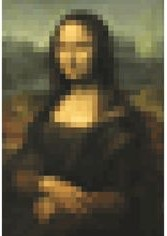
\includegraphics[width=4cm,height=5cm]{images/discrete/monalisa2.jpg}
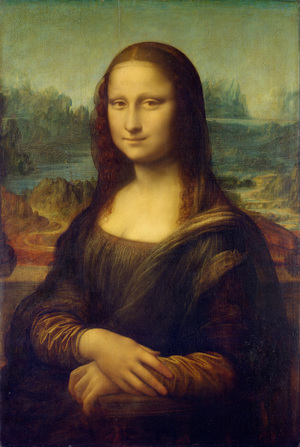
\includegraphics[width=4cm,height=5cm]{images/discrete/monalisa3.jpg}\\
{\captionfont Illustration of space discretisation. If the picture is cut up 
in a small number of cells covering it we obtain the picture on the left.
If more cells are used, we obtain the picture in the middle. When a (very) large
number of cells is used we finally see all details and it approaches a continuum.}
\end{center}


